
\subsection{L'Application Checkers}

l'application Checkers (principe), décompilation, un bytecode obscure
dex2jar, jd-gui, correction des erreurs, éclaircissement du code, une archi mvc.
Fonctionnement de l'appli en interne
\subsubsection{Principe}
\begin{figure}[hp]
	      \begin{center}
		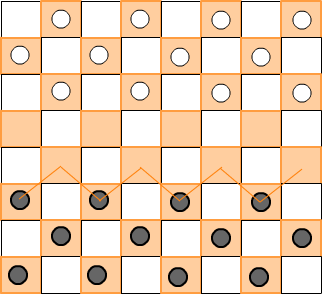
\includegraphics[scale=0.5]{principe}
	      \end{center}
	\legend{Principe}
\end{figure}

Le jeu est composé de 8 cases sur 8, c’est-à-dire 4 cases en moins que le jeu de dame classique.  Se joue en deux modes : utilisateur contre ordinateur ou utilisateur contre utilisateur.\\
Un joueur peut choisir une couleur (des pions/dames noires ou des pions/dames blanche).  Le jeu est initialement constitué de 3 lignes de 4 pions espacés d’une case. Chaque pion/dame peut se déplacer en diagonale. 
Une dame ou un pion peut faire une prise en faisant un déplacement en diagonal. Le jeu oblige à faire une prise (Must capture) si l'utilisateur n'a pas activé l'option capture optionnelle. 
Un pion se déplace uniquement en avant et se transforme en une dame (K) lorsqu’il arrive à la dernière ligne du camp de l’adversaire. Une dame peut effectuer une prise en faisant un déplacement en arrière ou en avant\\
Un joueur est désigné gagnant si l’adversaire ne possède plus de dames ou de pions.

\subsubsection{Décompilation et analyse du code}

Afin de pouvoir analyser le code de l'application plus aisément, nous avons dû trouver un moyen de décompiler l'application vers du code java.
Pour ce faire, nous avons utilisé \textit{dex2jar} \cite{dex2jar},
une api permettant de décompiler un fichier apk en un fichier jar contenant des fichiers class.
Ensuite, nous avons dû utiliser \textit{jd-gui} \cite{jdgui} sur ce fichier jar pour en afficher le code source.
L'application permet d'exporter les sources ainsi décompilées.

Une fois le code java de l'application en notre possession, nous avons pu commencer à l'analyser.
Nous avons vite remarqué que le code avait été obscurcit avant d'être compilé par le développeur de l'application.
Cela signifie que toutes variables et fonctions avaient un nom sans aucun sens, ce qui gêna la compréhension du code.
Nous avons aussi remarqué que la décompilation c'était mal passée à cause de return et de break à des endroits incongrus.
Nous avons donc commencé par supprimer ces erreurs afin de pouvoir avoir un code "compilable" sous Eclipse.
Ceci nous a offert un accès à l'outil de refactorisation de code pour renommer les variables après avoir compris à quoi elles pouvaient servir.

Malgré cela, à cause du problème de décompilation, certaines méthodes n'avaient aucun sens.
Nous avons donc décidé de relire le code smali des méthodes correspondantes afin de le traduire manuellement en java et ainsi avoir le code original exact.

\subsubsection{Architecture}
Dans un point de vue général, le développeur du jeu Checkers a adopté une architecture MVC. Ce qui nous a beaucoup aidé à determiner les différentes 
classes. 
\begin{figure}[hp]
	      \begin{center}
		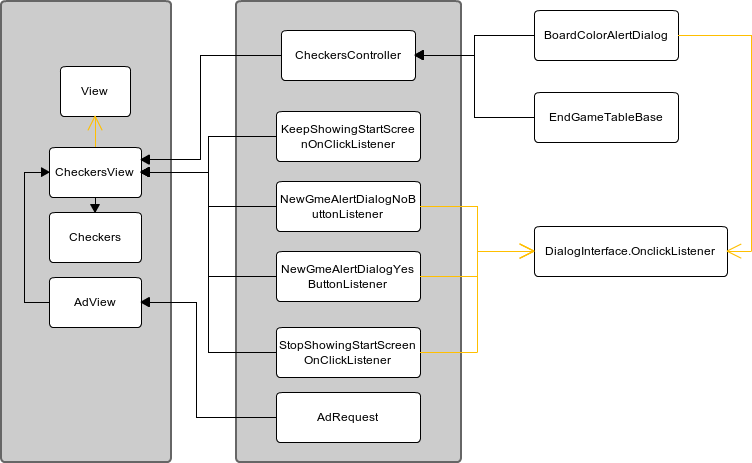
\includegraphics[scale=0.6]{archi}
	      \end{center}
	\legend{architecture}
\end{figure}
La classe Checkers est la classe principale de l’application.
La classe CherckersView (b.smali) hérite de la classe android.view.View qui gére les vues de l’application. La classe AdView gère la vue pour la publicité.
CheckersController (a.smali) est le controleur principal de l’application. Les classes KeepShowingStartScreenOnclickListener (e.smali), NewGameAlertDialogNoButtonListener (d.smali), NewGameAlertDialogYesButtonListener (c.smali) et StopShowingStartScreenOnclickListener (f.smali) implémente l'interface DialogInterface.OnclickListener sont les classes qui gère les clics.
AdRequest est la classe qui est responsable du chargement de la publicité.
